% Latex template: https://github.com/mqTeXUsers/Macquarie-University-Beamer-Theme

% Slide Masters:

% Title
% Text
% 2 column
% Full-image
% Bibliography
% Closing
 
\documentclass[aspectratio=169, 11pt]{beamer} % Aspect ratio
% https://tex.stackexchange.com/a/14339/5483 
% Possible values: 1610, 169, 149, 54, 43 and 32.
% 169 = 16:9

\PassOptionsToPackage{table}{xcolor}    %https://tex.stackexchange.com/a/5365/5483

\usetheme{macquarie}
\usepackage{multicol} % https://tex.stackexchange.com/a/396018/5483
\usepackage{xurl}
\usepackage[british]{babel}       % Set language
% \usepackage[utf8x]{inputenc}      % Set encoding
\usepackage{colortbl}
\mode<presentation>           % Set options
{
  \usetheme{default}          % Set theme
  \usecolortheme{default}         % Set colors
  \usefonttheme{default}          % Set font theme
  \setbeamertemplate{caption}[numbered] % Set caption to be numbered
}

% Uncomment this to have the outline at the beginning of each section highlighted.
%\AtBeginSection[]
%{
%  \begin{frame}{Outline}
%    \tableofcontents[currentsection]
%  \end{frame}
%}

\usepackage{graphicx}         % For including figures
\usepackage{booktabs}         % For table rules
\usepackage{hyperref}         % For cross-referencing


\usepackage{enumitem} % https://tex.stackexchange.com/a/2292/5483

%https://tex.stackexchange.com/a/371844/5483
\setbeamerfont{bibliography entry author}{size=\tiny}
\setbeamerfont{bibliography entry title}{size=\tiny}
\setbeamerfont{bibliography entry location}{size=\tiny}
\setbeamerfont{bibliography entry note}{size=\tiny}
\setbeamerfont{bibliography item}{size=\tiny}

%https://tex.stackexchange.com/q/333587/5483
%TODO SHAWN REPLACE OSF URL
%\setbeamertemplate{footline}{\strut~\texttt{https://osf.io/v5jp7/}\hfill\insertframen%umber~/~\inserttotalframenumber\strut~~~}

\title{`Trust but verify': Transparency \& compliance} % Presentation title
\author{A/Prof Shawn A Ross, Director of Data Science and eResearch}               % Presentation author
\institute{Office of the Deputy Vice-Chancellor (Research)}         % Author affiliation
\date{Tuesday 10 September 2019}                 % Today's date  
\begin{document}

% Title page
% This page includes the informations defined earlier including title, author/s, affiliation/s and the date
% \begin{frame}[noframenumbering]

%Abstract: Since the recognition of the 'reproducibility crisis' a decade ago, research technologies have been proposes as part of the solution. What began as recommendations or guides to best practice have evolved into publisher and funder mandates, and have influenced codes of ethical practice. The Findable, Accessible, Interoperable, and Reusable (FAIR) data principles and the Transparency and Openness Promotion (TOP) guidelines have been among the most influential. Both have been endorsed by funders and publishers, and are poised to change research practice beyond the early adopters already implementing them. To void marginalisation - the inability to publish in quality outlets or compete for major grants - researchers from across disciplines are facing significant change to daily practice, requiring much more technical literacy and computational thinking ability than most now possess. The transformation of research requires retraining of mid-career and senior researchers, but will likely depend upon training younger researchers, even in disciplines where such training is not customary.


\maketitle

  
% \end{frame}

% Outline
% This page includes the outline (Table of content) of the presentation. All sections and subsections will appear in the outline by default.
\begin{frame}{The context of Research Data Management}
  \tableofcontents
\end{frame}

% The following is the most frequently used slide types in beamer
% The slide structure is as follows:
%
%\begin{frame}{<slide-title>}
% <content>
%\end{frame}


% Presentation providing context for the new data governance policies and procedures at Macquarie University

\section{Transparency and reproducibility}

\begin{frame}{The `reproducibility crisis'}
  For nearly a decade the reproducibility crisis has featured in the scientific literature \cite{Jasny2011-bw, Baker2016-cf, Munafo2017-bj}. Low reproducibility rates have emerged from large-scale studies:
    \begin{itemize}[label=\textbullet]
        \item Results from only 39\% of psychology studies could be reproduced \cite{Open_Science_Collaboration2015-vf}.
        \item Even lower reproducibility rate in biomedical research \cite{Begley2012-xt,Prinz2011-za}.
    \end{itemize}
\end{frame}

\begin{frame}{Perceptions of the reproducibility crisis}
  \begin{figure}[H]
    \centering
        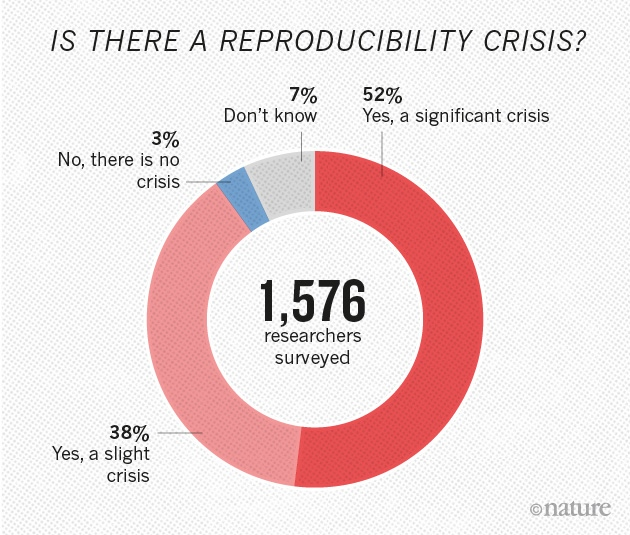
\includegraphics[height=.7\textheight]{figures/reproducibility-graphic-online1.jpeg}
        \caption{Is there a reproducibility crisis? \cite{Baker2016-cf}}
        \label{fig:Baker2016}
  \end{figure}
\end{frame}

\begin{frame}{Motivation: Preserving data}
 \begin{figure}[H]
    \centering
        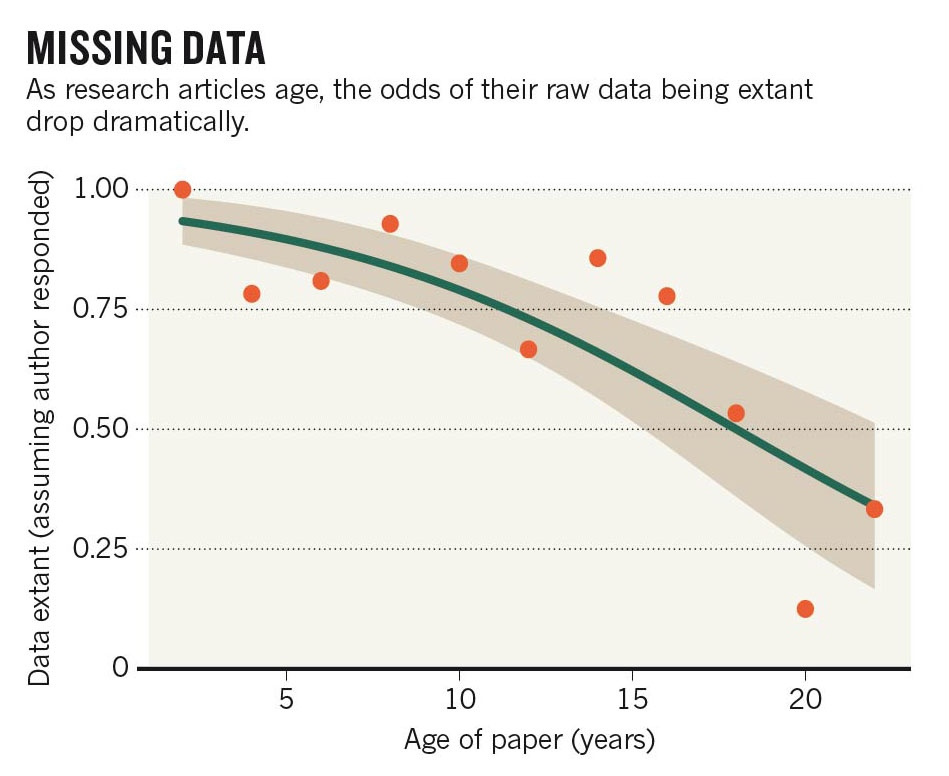
\includegraphics[height=.75\textheight]{figures/Missing-Data.png}
        \caption{\cite{Vines2014-zr}}
        \label{fig:vines2014}
 \end{figure}
\end{frame}

\begin{frame}{The response: calls for rigour and transparency}
  Manifestos, statements, and guidelines:
    \begin{itemize}[label=\textbullet]
        \item Early example: OECD Priniples and Guidelines for Access to Research Data \cite{Oecd2007-vi}.
        \item Findable, Accessible, Interoperable, and Reusable (FAIR) data \cite{Wilkinson2016-mr, Go-fair2017-vs}.
        \item Transparency and Openness Promotion (TOP) guidelines \cite{Nosek2015-wm, Cos2019-mr}.
        \item Data transparency toolkit \cite{Perkel2018-rw}.
    \end{itemize}
\end{frame}

\section{From guidelines to mandates}

\begin{frame}{Journal transparency mandates}
  Mandates for transparency or reproducibility:
    \begin{itemize}[label=\textbullet]
        \item Nature: Transparency Upgrade \cite{Nature2017-lq}.
        \item Nature: FAIR data in Earth science \cite{Nature2019-ng}.
        \item Copernicus: FAIR data in atmospheric sciences \cite{Van_Edig2018-bu}.
        \item TOP Guidelines signatories include publishers representing 1000+ journals, as well as professional organisations and major private foundations  \cite{Cos2019-mr}.
    \end{itemize}
\end{frame}

% https://tex.stackexchange.com/a/2292/5483
% https://ctan.org/pkg/enumitem?lang=en

\begin{frame}{Level 2 TOP Guidelines for authors (excerpt)}
  
    \begin{enumerate}[label=\arabic*.]
        \setcounter{enumi}{1}
        % This increments the enumerate counter by 1.
        
        \item Authors using original data must:
        \begin{enumerate}[label=\alph*.]
            \item make the data available at a trusted digital repository [...]
            \item include all variables, treatment conditions, and observations described in the manuscript.
            \item provide a full account of the procedures used to collect, preprocess, clean, or generate the data.
            \item provide program code, scripts, codebooks, and other documentation sufficient to precisely reproduce all published results.
            \item provide research materials and description of procedures necessary to conduct an independent replication of the research.
        \end{enumerate}
    \end{enumerate}
    \cite{Osf2014-pf}
\end{frame}

\begin{frame}{TOP Guidelines: publisher adoption}
  \begin{figure}[H]
    \centering
        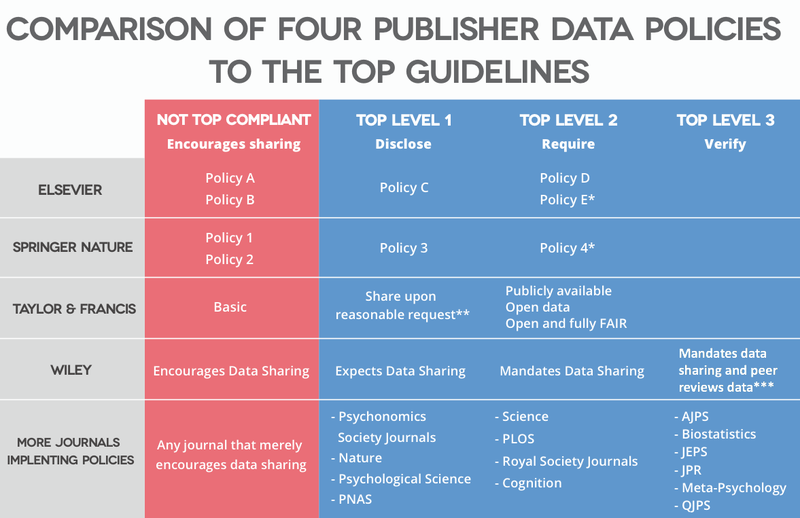
\includegraphics[height=.7\textheight]{figures/TOP-landscape.png}
        \caption{The Landscape of Open Data Policies \cite{Mellor2018-bf}}
        \label{fig:figure2}
  \end{figure}
\end{frame}

\begin{frame}{TOP Guidelines: funder endorsement}
  Private funders have endorsed via the Open Funders Research Group:
    \begin{itemize}[label=\textbullet]
        \item Alfred P. Sloan Foundation
        \item American Heart Association
        \item Bill and Melinda Gates Foundation
        \item Howard Hughes medical Institute
        \item John Templeton Foundation
        \item Laura and John Arnold Foundation
        \item Open Society Foundations
        \item Robert Wood Johnson Foundation
        \item Wellcome Trust
        \item and six more \cite{Ofrg2019-pq}
    \end{itemize}
\end{frame}

\begin{frame}{Other Funder data policies}
  \begin{figure}[H]
    \centering
        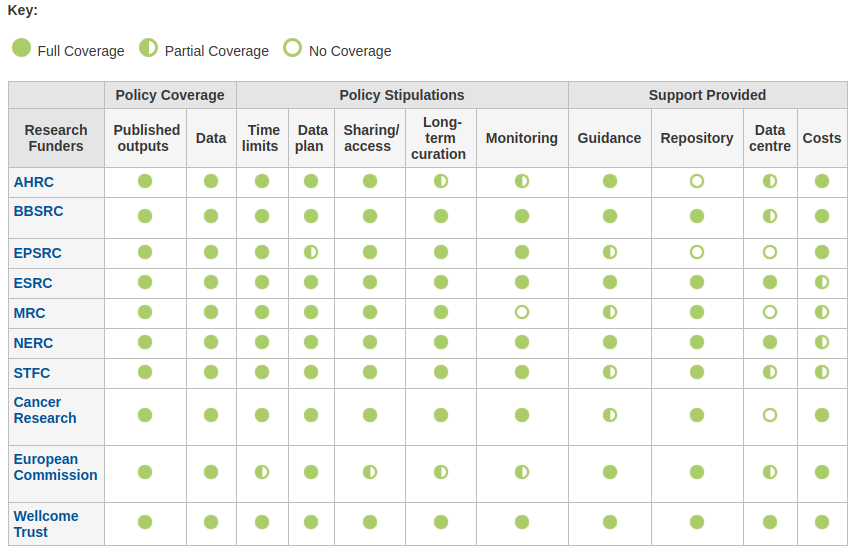
\includegraphics[height=.7\textheight]{figures/DCC-Funders.png}
        \caption{Overview of funders' data policies \cite{Dcc2019-jn}}
        \label{fig:Dcc2018}
  \end{figure}
\end{frame}

\begin{frame}{Not just the natural sciences}
  Changes are coming to HASS disciplines:
    \begin{itemize}[label=\textbullet]
        \item American Journal of Political Science requires (and tests) data and code \cite{Jacoby2017-lw, Ajps2015-ex}.
        \item All European Academies (allea) E-Humanities working group \cite{Allea2019-wy} has issued an Open Consultation on `Sustainable and FAIR Data Sharing in the Humanities' \cite{Allea2019-aw}.
        \item Research Data Alliance (RDA) has an 'Ambassador for the Humanities' and is examining how RDA standards and outputs can apply to humanities disciplines \cite{Rda2019-wc}.
    \end{itemize}
\end{frame}

\begin{frame}{EU research governance policy}
  With the Horizon 2020 program \cite{European_Commission2019-an} Europe made 'research data open by default':
    \begin{itemize}[label=\textbullet]
        \item Opt-outs: 'as open as possible, as closed as necessary'.
        \item Continuing investment, e.g., FAIRsFAIR project \cite{Knaw-dans2019-sv} to implement FAIR across repositories.
    \end{itemize}
\end{frame}

\begin{frame}{Australia: Data sharing in the NHMRC Statement}
    The NHMRC `strongly encourages' data sharing in the National Statement on Ethical Conduct in Human Research and their Open Access Policy. \cite{Nhmrc2018-sj, Nhmrc2018-vn} \par
    National Statement 3.1.50 \par
    In the absence of justifiable ethical reasons (such as respect for cultural ownership or unmanageable risks to the privacy of research participants) and to promote access to the benefits of research, researchers should collect and store data or information generated by research projects in such a way that they can be used in future research projects. Where a researcher believes there are valid reasons for not making data or information accessible, this must be justified.
\end{frame}

\begin{frame}{NHMRC Open Access Policy 2018 changes}
    Key changes to the Open Access Policy (15 January 2018) \par
    Research data and metadata (2.2) \par
    NHMRC now strongly encourages researchers to take reasonable steps to share research data and associated metadata arising from NHMRC supported research.\par
    FAIR principles (2.7) \par
    Reference to the Australian F.A.I.R. principles (Findable, Accessible, Interoperable, Reusable) when publishing research literature and sharing data has been made.
\end{frame}

\begin{frame}{NHMRC Open Access Policy data sharing}
    Medatdata (4.1) \par
    The metadata for the peer-reviewed publication must be made openly accessible via an institutional repository as soon as possible but no later than 3 months from the date of publication. \par
    Data (4.2) \par
    NHMRC acknowledges the importance of making research data publicly accessible and therefore strongly encourages researchers to consider the reuse value of their data and to take reasonable steps to share research data and associated metadata arising from NHMRC supported research.
\end{frame}

\begin{frame}{Legal compliance}
    \begin{itemize}[label=\textbullet]
        \item NSW General Retention and Disposal Authority GDA 23; data associated with `significant' research or researchers must be kept forever (23.6.1) \cite{Nsw2015-kv}
        \item NSW Privacy and Personal Information Protection Act 1998 No 133, esp. Part 2, Division 1, Section 19, which flags indicators of high sensitivity and establishes data sovereignty.\cite{Nsw1998-mw} Compare the (Australian) Privacy Act 1988, esp. Part II, Division 1, Section 6 `Sensitive Information' and Schedule 1, and `Australian Privacy Principles', Section 8, which covers some university-controlled entities. \cite{Ag2017-oz,Oaic2019-ng}
        \item NSW Notifiable Data Breach guidance \cite{Ipc_nsw2018-yr}; see also the Australian Notifiable Data Breaches scheme \cite{Oaic2019-dq}
        \item EU General Data Protection Regulation \cite{Gdpr2019-ee}
    \end{itemize}
\end{frame}

\section{Beyond compliance}

\begin{frame}{Large-scale research}
    The same approaches that facilitate transparency and reproducibility support the kind of scalable and synthetic research that can address archaeological `grand challenges'. \cite{Kintigh2014-ub}
        \begin{itemize}[label=\textbullet]
            \item Paper data capture and manual digitisation and cleaning don't scale.
            \item Collaboration based on email and desktop software doesn't scale.
    \end{itemize}
\end{frame}

\begin{frame}{Scalable approaches to data and analysis}
  \begin{figure}[H]
    \centering
        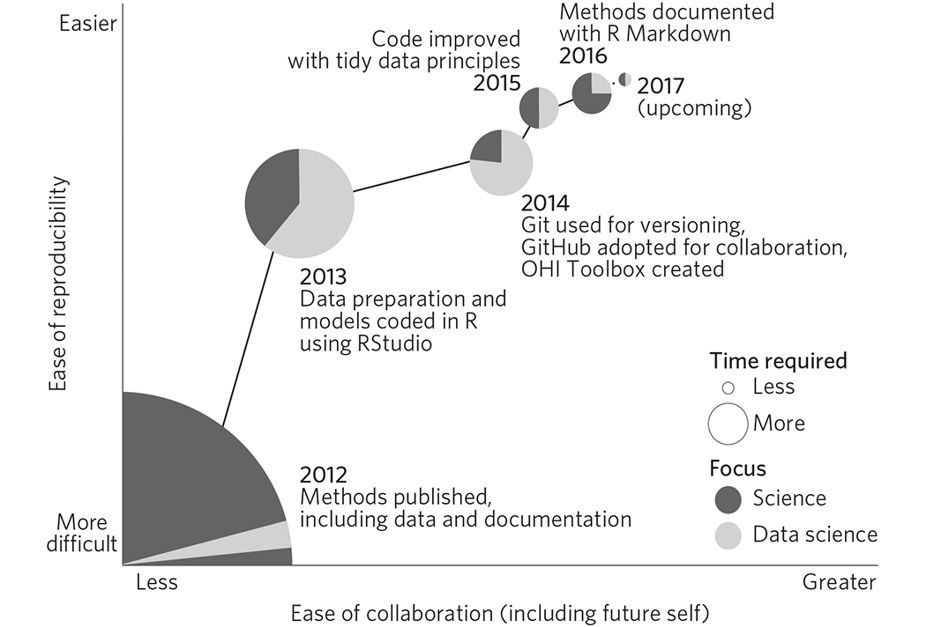
\includegraphics[height=.7\textheight]{figures/Ocean-Health-Index.jpg}
        \caption{Better science in less time, illustrated by the Ocean Health Index project. \cite{Stewart_Lowndes2017-lj}}
        \label{fig:stewart_lowndes}
  \end{figure}
\end{frame}

\section{From current practice to better practice}

\begin{frame}{What does this mean? Are we ready?}
  Emerging good practice - and publisher and funder policies - mean:
    \begin{itemize}[label=\textbullet]
        \item Comprehensive, FAIR datasets will be deposited in domain-specific repositories. Data, and especially metadata, quality will be higher.
        \item Data will be captured digitally as early in research as possible, and provenance / version history maintained.
        \item Research approach, processes, and procedures will be documented.
        \item Data processing and analysis will use code (not Excel!) 
        \item Code will be documented and published for reuse.
        \item Further steps taken for analytical reproducibility (use of OSS, version control, automation, containerisation, etc.). 
    \end{itemize}
\end{frame}

\begin{frame}{Challenges and paths forward}
  How do we get from where we are now to where we want to be?
      \begin{itemize}[label=\textbullet]
        \item Understand the evolving expectations of transparent research. 
        \item Pursue proper training
        \item Look past desktop software (Excel, ARCGIS, Filemaker, Access, etc.).
        \item Use emerging research- and domain-specific solutions (even if imperfect).
        \item Overcome `not invented here'; if a solution exists, use it.
        \item Budget for `ground-up' transparency (data and code). Up-front costs will be high but offer longer-term payoffs (in costs, time, and quality).
        \item Implement (and budget for) fundamental good practice in data and code management before other technologies.
        \item Improve research design (prioritise approach over methods) \cite{Muthukrishna2019-kt, Hole1973-cy}
    \end{itemize}
\end{frame}
% \bibliographystyle{apalike}

% Adding the option 'allowframebreaks' allows the contents of the slide to be expanded in more than one slide.
% The "1" comes from the outer theme"

\section{References}

\begin{multicols}{2}[]
\bibliography{references}
\bibliographystyle{apalike}
\end{multicols}


% \begin{frame}[allowframebreaks]{References}
  
%   \bibliography{references}
%   \bibliographystyle{apalike}
% \end{frame}


\begin{frame}{Thank you!}

% This presentation is available at:
% \texttt{https://osf.io/...}

Source code for this presentation is available at: \texttt{https://github.com/saross/Research-Transparency}

This work is licensed under a Creative Commons Attribution 4.0 International License.

\end{frame}



\end{document}